\documentclass{article}
\usepackage[utf8]{inputenc}
\usepackage{../lambdatex} %disponibile all'indirizzo http://lambdamath.altervista.it/esercizi/lambdatex.sty

\everymath{\displaystyle}
\title{Università degli Studi di Trento - Dipartimento di Matematica\\
CdL in Matematica – a.a. 2022–2023\\ Note esercitazione}
\author{Esercitatore: Simone Verzellesi\thanks{Trascrizione a cura di Davide Borra e Matilde Calabri}}
\date{03 Ottobre 2022}

\begin{document}
\maketitle
\lhead{Note esercitazione}
\chead{Università degli Studi di Trento - Dipartimento di Matematica\\
CdL in Matematica – a.a. 2022–2023}
\rhead{03/10/2022}
\setlength{\headheight}{30pt}.
\begin{enumerate}[label=\textbf{Esercizio 3.\arabic*.},itemindent=*]
%%%%%%%%%%%%%%%%%%%%%%%%%%%%%%%%%%%%%%%%%%%%%%%%%%%%%
    \item Determinare gli estremi inferiore e superiore ed eventuali massimi e minimi dei seguenti insiemi 
    \begin{enumerate}
        \item $A=\left\{\frac{n}{n+1},n\in \N\right\}$
        \item $B=\left\{2(-1)^n-\frac{1}{2n}, n\in \N\setminus \{0\}\right\}$
        \item $C=\left\{\frac{n}{m}: n, m\in \N\setminus\{0\},n>m\right\}$
    \end{enumerate}
    \item[\textit{\large Soluzione~}]~
    \begin{enumerate}
        \item \begin{oss}
            Possiamo riscrivere $\frac{n}{n+1}=\frac{n+1-1}{n+1}=1-\frac{1}{n+1}$.
        \end{oss}
        Se calcoliamo alciuni elementi dell'insieme $A=\left\{0, \frac{1}{2}, \frac{2}{3}, \frac{3}{4},\dots\right\}$ ci accorgiamo che sono tutti compresi in $[0,1[$.\\
        \textbf{Estremo inferiore:} siccome $n\in \N$, $\frac{n}{n+1}\geq0\forall n\in \N$. Inoltre $0\in A$, per cui si ha che $\inf A=0$ e $\min A=0$.\\
        \textbf{Estremo superiore:} Dobbiamo dimostrare che $\sup A=1$
        \begin{itemize}
            \item $1\geq 1-\frac{1}{n+1}$ perché $\frac{1}{n+1}>0~~\forall n\in \N$
            \item Dobbiamo provare che $\forall \varepsilon >0, \exists n\in \N:\frac{n}{n+1}\geq 1-\varepsilon$. Fissiamo $\varepsilon$ e cerchiamo $n$: \[\frac{n}{n+1}\geq 1-\varepsilon~~~\Harr\]\[\cancel{1}-\frac{1}{n+1}=\cancel{1}-\varepsilon~~~\Harr\]\[(n+1)\varepsilon\geq 1~~~\Harr\]\[n\varepsilon\geq 1-\varepsilon ~~~\Harr\]\[n\geq \frac{1-\varepsilon}{\varepsilon}\]
            Se $\varepsilon \geq 1$, la disequazione è sempre verificata perché il numeratore diventa negativo. \\Se $varepsilon<1$ basta scegliere un numero naturale $n>\frac{1-\varepsilon}{\varepsilon}$.\\Questo dimostra che $\sup A=1$. L'insieme non ammette massimo perché $1\notin A$.
        \end{itemize}
        \item Separiamo i casi in cui $n$ è pari da quelli in cui $n$ è dispari:
        \[B=\underbrace{\left\{2-\frac{1}{2n}, \in \N \text{ e }n\text{ pari}\right\}}_{B'}\cup\underbrace{\left\{-2-\frac{1}{2n}, \in \N \text{ e }n\text{ dispari}\right\}}_{B''}\]
        \begin{oss}
            È un'unione disgiunta, cioè $\forall x \in B', y\in B'', y<0<x$, infatti 
                \[2-\frac{1}{2n}>0\text{~~ e ~~}-2-\frac{1}{2n}<0\]
            Da questo si ottiene che $\sup B=\sup B'$ e $\inf B=\inf B''$     
        \end{oss}
        \textbf{Estremo superiore:}
        \begin{oss}
            In $B'$ gli elementi si avvicinano a 2 quando $n$ cresce perché $\frac{1}{2n}$ diventa sempre più piccolo. 
        \end{oss}
        La dimostrazione è analoga a quella del $\sup A$.\\
        \textbf{Estremo inferiore:}\\
        Calcoliamo alcuni degli elementi di $B=\left\{-\frac{5}{2},-\frac{13}{6},\dots\right\}$. Si nota che all'aumentare di $n$ gli elementi di $B''$ crescono, di conseguenza si ha $\inf B=\min B''= -\frac{5}{2}$.
        \item \textbf{Estremo superiore:}
        \begin{oss}
            Se pongo $m=1$, ottengo $\N_{\geq2}$. Di conseguenza $\N_{\geq2}\subseteq C$. Da questo si ricava che $\sup C\geq \sup \N_{\geq 2}$, da cui (siccome $\sup \N_{\geq 2}=+\infty$), \[\sup C=+\infty\]
        \end{oss}
        \textbf{Estremo inferiore:}\\
        Scelgo $m=n+1$, ottengo $D=\left\{\frac{n+1}{n}, n\neq 0\right\}\subseteq C$. Analogamente a quanto fatto nel punto (a) è possibile dimostrare che $\inf D=1$. Inoltre siccome $D\subseteq C$, si ha $\inf D\geq \inf C\Rarr \inf C\leq 1$. Inoltre sappiamo che $\forall n> m, \frac{n}{m}>1$, di conseguenza $\inf C\geq 1$. Siccome $\inf C\geq 1$ e $\inf C \leq 1$, si ha $\inf C=1$.
    \end{enumerate}
    
%%%%%%%%%%%%%%%%%%%%%%%%%%%%%%%%%%%%%%%%%%%%%%%%%%%%%
    \item Risolvere in $\C$ le seguenti equazioni: 
        \begin{enumerate}
            \item $\frac{1}{|z|\cdot \overline{z}}=\cos\frac{\pi}{4}+i\sen \frac{\pi}{4}$
            \item $\overline{z}(\Im z-\Re z)=z$
            \item $2z^2+\overline{z}=-1$
        \end{enumerate}

    \item[\textit{\large Soluzione~}]~
        \begin{enumerate}
        
        
        \item
        \[\frac{1}{|z|\cdot \overline{z}}=\cos\frac{\pi}{4}+i\sen \frac{\pi}{4}~~~\Rarr\]
        \[\frac{1}{||z|\cdot\overline{z}|}=|\cos\frac{\pi}{4}+i\sen\frac{\pi}{4}|~~~\]
        Analizzo la prima parte dell'equazione
        \[\frac{1}{||z|\cdot\overline{z}}=\frac{1}{|z|\cdot|\overline{|z|}|}=\frac{1}{|z|^2}=1\Leftrightarrow|z|^2=1\Leftrightarrow |z|=1\]

        Torno all'equazione originale
        \[\frac{1}{\overline{z}}=\cos\frac{\pi}{4}+i\sen \frac{\pi}{4}\]
        Analizzo la prima parte dell'equazione
        \[\frac{1}{\overline{z}}=\frac{z}{z\cdot\overline{z}}=\frac{z}{|z|^2}\]
        Ritorno all'equazione originale e sfrutto il fatto che $|z|=1$
        \[z=\cos\frac{\pi}{4}+i\sen \frac{\pi}{4}\]
    

        \item $\overline{z}(\Im z-\Re z)=z$
        \par Utilizzo la forma algebrica $(z=a+ib)$
        \[(a-ib)(b-a)=a+ib~~~\Harr\]\[a(b-a)+ib(a-b)=a+ib~~~\Harr\]
        \[\begin{cases}
        a(b-a)=a \\ b(a-b)=b
        \end{cases} \]
        \par
        Distinguo due casi: \par
        Caso $a=0$
        \par
        \[\begin{cases}
        \forall b \\ -b^2=b\Leftrightarrow b(b+1)=0\Leftrightarrow z_1=0,z_2=-i
        \end{cases}\] 
        \par Caso $a\neq 0$
        \par
        \[\begin{cases}
        b-a=1\Leftrightarrow a-b=-1 \\ -b=b\Leftrightarrow b=0
        \end{cases} \Leftrightarrow a=-1\Leftrightarrow z_3=-1\]
        

        \item $2z^2+\overline{z}=-1$
        \par Utilizzo la forma algebrica $(z=a+ib)$
        \[2(a+ib)(a+ib)+(a-ib)=-1\Leftrightarrow 2a^2-2b^2+4abi+a-ib=-1\]
        \[\begin{cases}
        2a^2-2b^2+a=-1 \\ 4ab-b=0\Leftrightarrow b(4a-1)=0
        \end{cases}\]
        
        Distinguo due casi
        
        Caso $b=0$
        \[\begin{cases}
        2a^2+a+1=0 \\ \forall a
        \end{cases} \Leftrightarrow a_{1,2}=\frac{-1\pm\sqrt{1-8}}{4}\Leftrightarrow\nexists a\]
         Se b=0 non abbiamo soluzioni
        
        \par Caso $b\neq0$
        \par Dalla seconda equazione ottengo che $a=\frac{1}{4}$
        \[\begin{cases}
        2\cdot{\frac{1}{16}}-2b^2+\frac{1}{4}=-1 \\ a=\frac{1}{4}
        \end{cases}\Leftrightarrow -b^2=-\frac{11}{16}\Leftrightarrow b=\pm \frac{\sqrt{11}}{4}\]
         Ottengo quindi le soluzioni $z_{1,2}=\frac{1}{4}\pm\frac{\sqrt{11}}{4}$
    
    \end{enumerate}
    
%%%%%%%%%%%%%%%%%%%%%%%%%%%%%%%%%%%%%%%%%%%%%%%%%%%%%
    \item Si considerino le funzioni $f, g, h: \C\to\C$ definite come \[f(z)=z+z_0 \text{, ~~ con $z_0\in \C$ fissato}\]
    \[g(z)=iz\]
    \[h(z)=z^2\]
    e gli insiemi \[A=\{z: 0\leq \Re z \leq 1 \text{ e } 0\leq \Im z \leq 1\}\]
    \[B=\left\{z:|z|\leq 2, \arg z\in \left]\frac{3}{8}\pi, \frac{\pi}{2}\right[\right\}\]
    \[C=\{z:1\leq |z|\leq 2\}\]
    Rappresentare $f(A), g(B), h(B), h(C)$.
    \item[\textit{\large Soluzione~}] Prima di tutto rappresentiamo gli insiemi $A$, $B$, $C$ (Vedi Figura \ref{fig1}).
     \begin{figure}[h!]
        \centering
        \begin{subfigure}{0.3\textwidth}
            \definecolor{zzttqq}{rgb}{0.6,0.2,0.}
            \begin{tikzpicture}[line cap=round,line join=round,>=triangle 45,x=2cm,y=2cm]
                \begin{axis}[
                x=2.0cm,y=2.0cm,
                axis lines=middle,
                ymajorgrids=true,
                xmajorgrids=true,
                xmin=-0.6,
                xmax=1.6,
                ymin=-0.6,
                ymax=1.6,
                xtick={-0.5,0.0,...,1.5},
                ytick={-0.5,0.0,...,1.5},]
                \clip(-0.6,-0.6) rectangle (1.6,1.6);
                \fill[line width=2.pt,color=zzttqq,fill=zzttqq,fill opacity=0.10000000149011612] (0.,1.) -- (0.,0.) -- (1.,0.) -- (1.,1.) -- cycle;
                \draw [line width=2.pt,color=zzttqq] (0.,1.)-- (0.,0.);
                \draw [line width=2.pt,color=zzttqq] (0.,0.)-- (1.,0.);
                \draw [line width=2.pt,color=zzttqq] (1.,0.)-- (1.,1.);
                \draw [line width=2.pt,color=zzttqq] (1.,1.)-- (0.,1.);
                \draw (0.29307222648774567,0.9178337611061765) node[anchor=north west] {$A$};
                \end{axis}
                \end{tikzpicture}
                \caption{}
        \end{subfigure}
        \begin{subfigure}{0.3\textwidth}
            \definecolor{zzttqq}{rgb}{0.6,0.2,0.}
            \definecolor{qqwuqq}{rgb}{0.,0.39215686274509803,0.}
            \begin{tikzpicture}[line cap=round,line join=round,>=triangle 45,x=1.0cm,y=1.0cm, scale = 1.1]
            \begin{axis}[
            x=1.0cm,y=1.0cm,
            axis lines=middle,
            ymajorgrids=true,
            xmajorgrids=true,
            xmin=-1.5,
            xmax=2.5,
            ymin=-1.5,
            ymax=2.5,
            xtick={-1.0,0.0,...,2.0},
            ytick={-1.0,0.0,...,2.0},]
            \clip(-1.5,-1.5) rectangle (2.5,2.5);
            \draw [line width=2.pt,color=qqwuqq,fill=qqwuqq,fill opacity=0.10000000149011612] (0,0) -- (0.:0.3741774256653813) arc (0.:67.5:0.3741774256653813) -- cycle;
            \draw [line width=2.pt,color=zzttqq,fill=zzttqq,fill opacity=0.10000000149011612]  (0,0) --  plot[domain=1.1780972450961724:1.5707963267948966,variable=\t]({1.*2.*cos(\t r)+0.*2.*sin(\t r)},{0.*2.*cos(\t r)+1.*2.*sin(\t r)}) -- cycle ;
            \draw [color=qqwuqq](0.4888435380798806,0.8070387323953816) node[anchor=north west] {$\vartheta =\frac{3}{8}\pi$};
            \draw (0.05,1.5553935837261437) node[anchor=north west] {$B$};
            \end{axis}
            \end{tikzpicture}
            \caption{}
        \end{subfigure}
        \begin{subfigure}{0.3\textwidth}
            \definecolor{qqqqff}{rgb}{0.,0.,1.}
            \begin{tikzpicture}[line cap=round,line join=round,>=triangle 45,x=1.0cm,y=1.0cm]
            \begin{axis}[
            x=1.0cm,y=1.0cm,
            axis lines=middle,
            ymajorgrids=true,
            xmajorgrids=true,
            xmin=-2.5,
            xmax=2.5,
            ymin=-2.5,
            ymax=2.5,
            xtick={-2.0,-1.0,...,2.0},
            ytick={-2.0,-1.0,...,2.0},]
            \clip(-2.5,-2.5) rectangle (2.5,2.5);
            \filldraw [even odd rule, line width=2.pt,color=qqqqff,fill=qqqqff,fill opacity=0.10000000149011612] (0,0) circle (2) (0,0) circle (1);
            \node[color=qqqqff] at (1,1) {$C$};
            \end{axis}
            \end{tikzpicture}
            \caption{}
        \end{subfigure}
        \caption{}
        \label{fig1}
    \end{figure}
    Per come funziona la somma in $C$ (metodo punta-coda), sommare $z_0$ ad ogni punto dell'intervallo $A$ è come applicare alla rappresentazione dell'insieme una traslazione di vettore $v$ (Figura \ref{fig2}).\\
     \begin{figure}[h!] 
        \centering
        \definecolor{zzttqq}{rgb}{0.6,0.2,0.}
        \begin{tikzpicture}[line cap=round,line join=round,>=triangle 45,x=2.0cm,y=2.0cm]
        \begin{axis}[
        x=2.0cm,y=2.0cm,
        axis lines=middle,
        ymajorgrids=true,
        xmajorgrids=true,
        xmin=-0.37507864260047524,
        xmax=3.756772840196521,
        ymin=-0.40873055254144736,
        ymax=2.2923711155603104,
        xtick={-0.0,0.5,...,3.5},
        ytick={-0.0,0.5,...,2.0},]
        \clip(-0.37507864260047524,-0.40873055254144736) rectangle (3.756772840196521,2.2923711155603104);
        \fill[line width=2.pt,color=zzttqq,fill=zzttqq,fill opacity=0.10000000149011612] (0.,1.) -- (0.,0.) -- (1.,0.) -- (1.,1.) -- cycle;
        \fill[line width=2.pt,color=zzttqq,fill=zzttqq,fill opacity=0.10000000149011612] (2.,2.) -- (2.,1.) -- (3.,1.) -- (3.,2.) -- cycle;
        \draw [line width=2.pt,color=zzttqq] (0.,1.)-- (0.,0.);
        \draw [line width=2.pt,color=zzttqq] (0.,0.)-- (1.,0.);
        \draw [line width=2.pt,color=zzttqq] (1.,0.)-- (1.,1.);
        \draw [line width=2.pt,color=zzttqq] (1.,1.)-- (0.,1.);
        \draw [->,line width=2.pt] (0.,0.) -- (2.,1.);
        \draw [line width=2.pt,color=zzttqq] (2.,2.)-- (2.,1.);
        \draw [line width=2.pt,color=zzttqq] (2.,1.)-- (3.,1.);
        \draw [line width=2.pt,color=zzttqq] (3.,1.)-- (3.,2.);
        \draw [line width=2.pt,color=zzttqq] (3.,2.)-- (2.,2.);
        \draw (0.29217687636053036,0.919364566929013) node[anchor=north west] {$A$};
        \draw (2.4222618022745097,1.9010000900158752) node[anchor=north west] {$f(A)$};
        \begin{scriptsize}
        \draw[color=black] (1.398922809252583,0.6242323181577997) node {$z_{0}$};
        \end{scriptsize}
        \end{axis}
        \end{tikzpicture}
        \caption{}
        \label{fig2}
    \end{figure}
    Consideriamo un numero complesso $z$ in forma trigonometrica $z=|z|(\cos (\arg z)+ i \sen(\arg z))$. Il numero complesso $iz$ è \[iz=|i||z|\left(\cos\left(\arg z+\frac{\pi}{2}\right)+i\sen\left(\arg z+\frac{\pi}{2}\right)\right)\]
    Quindi è come se fosse stata applicata all'insieme una rotazione di $\frac{\pi}{2}$ (Figura \ref{fig3}).
     \begin{figure}[h!] 
        \centering
        \definecolor{qqwuqq}{rgb}{0.,0.39215686274509803,0.}
        \definecolor{zzttqq}{rgb}{0.6,0.2,0.}
        \definecolor{ududff}{rgb}{0.30196078431372547,0.30196078431372547,1.}
        \begin{tikzpicture}[line cap=round,line join=round,>=triangle 45,x=1.0cm,y=1.0cm]
        \begin{axis}[
        x=1.0cm,y=1.0cm,
        axis lines=middle,
        ymajorgrids=true,
        xmajorgrids=true,
        xmin=-2.754027484353424,
        xmax=2.334785504695761,
        ymin=-0.6771983894106297,
        ymax=2.6654532798667763,
        xtick={-2.0,-1.0,...,2.0},
        ytick={-0.0,1.0,...,2.0},]
        \clip(-2.754027484353424,-0.6771983894106297) rectangle (2.334785504695761,2.6654532798667763);
        \draw [line width=2.pt,color=zzttqq,fill=zzttqq,fill opacity=0.10000000149011612]  (0,0) --  plot[domain=1.1780972450961724:1.5707963267948966,variable=\t]({1.*2.*cos(\t r)+0.*2.*sin(\t r)},{0.*2.*cos(\t r)+1.*2.*sin(\t r)}) -- cycle ;
        \draw [color=qqwuqq](0.4888435380798802,0.8070387323953824) node[anchor=north west] {$\vartheta =\frac{3}{8}\pi$};
        \draw (0.12713869327001168,1.555393583726145) node[anchor=north west] {$B$};
        \draw [line width=2.pt,color=zzttqq,fill=zzttqq,fill opacity=0.10000000149011612]  (0,0) --  plot[domain=1.1780972450961724:1.5707963267948966,variable=\t]({0.*2.*cos(\t r)+-1.*2.*sin(\t r)},{1.*2.*cos(\t r)+0.*2.*sin(\t r)}) -- cycle ;
        \draw (-1.7188032733458691,0.5825322769961536) node[anchor=north west] {$g(B)$};
        \begin{scriptsize}
        \draw [fill=ududff] (0.,0.) circle (2.5pt);
        \draw[color=ududff] (0.08972095070347355,0.22706372261404137) node {$B$};
        \end{scriptsize}
        \end{axis}
        \end{tikzpicture}
        \caption{}
        \label{fig3}
    \end{figure}
    Analogamente si ha che siccome 
    \[z^2=|z|^2(\cos (2\arg z)+i\sen(2\arg z)\]
    Il raggio del settore circolare $h(B)$ è $4$ e l'angolo è in $\left]\frac{3}{4}\pi, \pi\right[$.
    \begin{proof}
        Dimostriamo che l'insieme \[S=\left\{z:|z|\leq4 \text{ e } \arg z \in \left]\frac{3}{4}\pi, \pi\right[\right\}\] coincide con $h(B)$. Per quanto detto in precedenza $h(b)\subseteq S$, quindi rimane da dimostrare che $h(b)\supseteq S$.\\
        Sia $z\in S: z=\rho (\cos \vartheta + i \sen \vartheta)$, bisogna dimostrare che $\exists w \in B:w^2=z$. Scegliamo \[w=\sqrt{\rho}\left(\cos\frac{\vartheta}{2}+ i \sen \frac{\vartheta}{2}\right)\], per il quale vale $h(w)=z$. Di conseguenza $z\in h(B)$, per cui $h(B)=S$.

    \end{proof}
    Analogamente si dimostra che $h(C)=\{z:1\leq |z|\leq 4\}$ (Figura \ref{fig4}).
     \begin{figure}[h!] 
        \centering
        \definecolor{qqqqff}{rgb}{0.,0.,1.}
        \begin{tikzpicture}[line cap=round,line join=round,>=triangle 45,x=1.0cm,y=1.0cm]
        \begin{axis}[
        x=1.0cm,y=1.0cm,
        axis lines=middle,
        ymajorgrids=true,
        xmajorgrids=true,
        xmin=-4.5,
        xmax=4.5,
        ymin=-4.5,
        ymax=4.5,
        xtick={-4.0,-3.0,...,4.0},
        ytick={-4.0,-3.0,...,4.0},]
        \clip(-4.5,-4.5) rectangle (4.5,4.5);
        \filldraw [even odd rule, line width=2.pt,color=qqqqff,fill=qqqqff,fill opacity=0.10000000149011612] (0,0) circle (4) (0,0) circle (1);
        \node[color=qqqqff] at (2,2) {$h(C)$};
        \end{axis}
        \end{tikzpicture}
        \caption{}
        \label{fig4}
    \end{figure}
%%%%%%%%%%%%%%%%%%%%%%%%%%%%%%%%%%%%%%%%%%%%%%%%%%%%%
\item Rappresentare i seguenti insiemi in $\mathbb{C}$
\begin{enumerate}
        \item $A=\left\{z:\frac{|z-1|}{|z+1|}=1\right\}$
        \item $B=\left\{z:|z-i-2|<|z+2|, |z|\geq 1\right\}$
    \end{enumerate}

\item[\textit{\large Soluzione~}]~
\begin{enumerate}
\item
$|z+1|\neq 0\Leftrightarrow z+1\neq 0\Leftrightarrow z\neq -1$\\
\(A=\left\{z\neq -1:|z-1|=|z+1|\right\}\)
$|z+1|=|z-(-1)|\Leftrightarrow |z-(-1)|=|z-1|$
\par $|z-(-1)|=$ distanza da $-1$, $|z-1|=$ distanza da $1$ (Figura \ref{fig5a})
\item
$|z-(i+2)|<|z-(-2)|$
\par Distanza da $i+2<$ distanza da $-2$ (Figura \ref{fig5b})
\begin{figure}[h!]
    \centering
    \begin{subfigure}{0.4\textwidth}
        \centering
        \definecolor{qqqqff}{rgb}{0.,0.,1.}
        \begin{tikzpicture}[line cap=round,line join=round,>=triangle 45,x=1.0cm,y=1.0cm]
        \begin{axis}[
        x=1.0cm,y=1.0cm,
        axis lines=middle,
        ymajorgrids=true,
        xmajorgrids=true,
        xmin=-3.3,
        xmax=3.3,
        ymin=-3.3,
        ymax=3.3,
        xtick={-3.0,-2.0,...,3.0},
        ytick={-3.0,-2.0,...,3.0},]
        \clip(-3.3,-3.3) rectangle (3.3,3.3);
        \draw [line width=2.pt,color=qqqqff] (0.,-3.3) -- (0.,3.3);
        \end{axis}
        \end{tikzpicture}
        \caption{}
        \label{fig5a}
    \end{subfigure}
    \begin{subfigure}{0.4\textwidth}
        \centering
        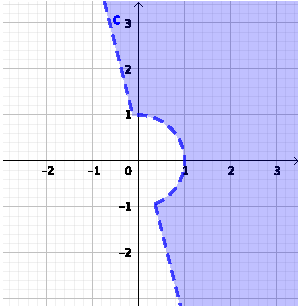
\includegraphics[width=\textwidth]{fig5b.pdf}
        \caption{}
        \label{fig5b}
    \end{subfigure}
    \caption{}
\end{figure}
\end{enumerate}

%%%%%%%%%%%%%%%%%%%%%%%%%%%%%%%%%%%%%%%%%%%%%%%%%%%%%
\item Dimostrare le seguenti disuguaglianze (con $a,b>0$).
\[\frac{2}{\frac{1}{a}+\frac{1}{b}}\underset{(i)}{\leq} \sqrt{ab}\underset{(ii)}{\leq}\frac{a+b}{2}\underset{(iii)}{\leq} \sqrt{\frac{a^2+b^2}{2}}\]

\item[\textit{\large Soluzione~}]~
\begin{enumerate}[label=(\textit{\roman*})]
    \item Riscriviamo il primo membro come \[\frac{2}{\frac{1}{a}+\frac{1}{b}}=\frac{2}{\frac{a+b}{ab}}=\frac{2ab}{a+b}\]
    Dobbiamo dimostrare che $\frac{2}{\frac{1}{a}+\frac{1}{b}}\leq \sqrt{ab}$\[\Harr ~~~\frac{2\sqrt{ab}}{a+b}\leq 1 ~~~\Harr~~~\sqrt{ab}\leq\frac{a+b}{2}\]
    Abbiamo dimostrato che la (\textit{i}) è equivalente alla (\textit{ii}), procediamo quindi alla dimostrazione di quest'ultima.
    \item \[\sqrt{ab}\leq\frac{a+b}{2}~~~\Harr~~~ab\leq\frac{a^2}{4}+\frac{b^2}{4}+\frac{1}{2}ab~~~\Harr~~~ \frac{a^2}{4}+\frac{b^2}{4}-\frac{1}{2}ab\geq 0~~~\Harr~~~\frac{1}{4}(a-b)^2\geq0\] 
    \item Dobbiamo dimostrare che $\frac{a+b}{2}\leq \sqrt{\frac{a^2+b^2}{2}}$
    \[\Harr ~~~ \frac{a^2}{4}+\frac{b^2}{4}+\frac{1}{2}ab\leq \frac{a^2+b^2}{2}~~~~\Harr~~~\frac{1}{4}(a-b)^2\geq 0\]
    \begin{lemma}[Disuguaglianza di Young]
        Siano $a,b, \varepsilon>0$, allora si ha che
        \[ab\leq \frac{1}{2}a^2+\frac{1}{2}b^2\]
        \[ab\leq \frac{\varepsilon}{2}a^2+\frac{1}{2\varepsilon}b^2\]
    \end{lemma}
\end{enumerate}
%%%%%%%%%%%%%%%%%%%%%%%%%%%%%%%%%%%%%%%%%%%%%%%%%%%%%
\end{enumerate}
\end{document}